\chapter{Conclusions and Future Work}
\label{ch:discussion_conclusion}

%\section{Discussion}
In this thesis, we have extensively explored and evaluated various state-of-the-art graph-based methods for approximate nearest neighbor (k-NN) search. The primary focus has been on understanding the effectiveness of graph-based indexing and search techniques, analyzing the core paradigms, and proposing new approaches to address existing challenges.

\section{Taxonomy of Graph Methods}
We proposed a comprehensive taxonomy that categorizes graph-based methods into five core paradigms: Seed Selection (SS), Neighborhood Propagation (NP), Incremental Insertion (II), Neighborhood Diversification (ND), and Divide-and-Conquer (DC). This taxonomy has helped to reveal the strengths and limitations of various methods by providing a clear classification scheme. Through this analysis, we identified that:
\begin{itemize}
    \item Methods based on incremental insertion scale better that their opponents on large datasets because each new insertion requires visiting each existing node in the graph only once. In contrast, methods that are not based on incremental insertion, e.g. NSG/SSG and Vamana, require two passes per existing graph node (for NSG/SSG, we count the indexing of the base graph as a first pass).
    \item Methods based on neighborhood diversification show the best search performance overall. This is because the efficient diversification of edges leads to pruning redundant directions in the graph,  thus facilitating the routing via long-range edges. This helps improve both indexing and search performance. The best neighborhood diversification technique is Relative Neighborhood Diversification (RND).
    %leading to the best search performance and edges pruning, thus reducing the index size.
    \item Methods based on the divide-and-conquer paradigm show a noticeable advantage on hard datasets. By dividing the data into smaller subsets, these methods can build a better quality proximity graph on each subset, as acquiring accurate nearest neighbors for each data point is challenging and the accuracy of the approximate nearest neighbor search during indexing is highly important and directly impacts the diversification of neighbors that can be achieved.

    %the smaller can paradigm nature in tackling the graph indexing in more granulary level, by dividing the data and building the proximity graphs on the small subsets, leads to better proximity graph when merged on hard datasets. 
    
    %This is true for hard datasets, seismic per example (dataset alone has high LID)
    %Another type of difficulty is OOD, where the dataset and query sets follows different distribution (cross model dataset per example), but the dataset itself has low LID (if we compute the LID based on the dataset points only)
    %For such datasets, to be honest we need first to make sense of what are the ground truths and if they are even making sense in there real values, recall accuracy or rbo may be misleading for such queries
    
\end{itemize}

Typically, state-of-the-art methods combine various building paradigms to achieve good performance. II-based and ND-based combinations generally show superior query performance, especially for large-scale datasets, while methods relying solely on NP struggle with scalability.

\section{State-of-the-Art Survey}
The study of state-of-the-art methods allowed us to identify the key factors influencing performance in graph-based indexing and search. Our study demonstrates varying performance trends across datasets of different sizes, query workloads of different hardness, and desired recall values. For small to medium-sized datasets (25GB and below), HNSW, NSG, and its improved version SSG consistently demonstrate excellent performance on easier datasets. On harder datasets, methods such as HCNNG, SPTAG, and ELPIS become the overall winners. As we scale to larger dataset sizes, methods like NSG and SSG face difficulty efficiently scaling, with only HNSW, VAMANA, and ELPIS able to handle datasets of 100GB and above effectively. We recommend ELPIS and HNSW for such sizes, as they provide the best performance trade-off between indexing and search.

\section{Study of Key Paradigms in Graph Indexing}
Our experiments show that Seed Selection (SS) and Neighborhood Diversification (ND) play a critical role in both indexing and query performance. The choice of SS strategies (such as KS, SN, and KD) directly impacts the efficiency of beam search. We found that SN and KS, particularly in large datasets, lead to more efficient search than methods like single fixed random entry point (SF). Moreover, ND methods such as RND and MOND offer substantial gains in both query accuracy and indexing time by reducing unnecessary edges, i.e. sparsifying the graph. Our results also show that ND-based approaches consistently outperform methods that do not incorporate neighborhood diversification. Notably, approaches such as RND and MOND have demonstrated significant improvements in search efficiency by effectively sparsifying the graph while maintaining good connectivity.

\section{Proposing an Approach Combining Tree and Graph-Based Methods}
One of the key contributions of this thesis is the proposal of ELPIS, a hybrid method that combines a divide-and-conquer approach with graph-based indexing. ELPIS divides the dataset into smaller clusters using a tree-based segmentation strategy (Hercules), and then constructs an HNSW graph within each cluster. This method addresses the scalability challenges of traditional graph-based approaches and reducing memory overhead. The results indicate that ELPIS achieves superior performance in terms of both indexing time and search latency, outperforming existing methods like HNSW and Vamana, particularly for large datasets.

\section{ELPIS for High-Latency Vector Search}
ELPIS was further adapted to handle high-latency vector search workloads by optimizing the trade-offs between cluster size and beam width. Our evaluation demonstrates that by dynamically adjusting the maximum leaf size and leveraging multi-threading, ELPIS can scale efficiently across varying dataset sizes and difficulty levels. ELPIS consistently achieves high recall and low query latency, even for hard-to-search datasets with high Local Intrinsic Dimensionality (LID) and low Local Relative Contrast (LRC).
\subsection{ELPIS+ for High-Throughput Vector Search}

We also proposed ELPIS+, an extension to ELPIS that supports high-throughput vector search.
%with larger leaf sizes, whereas it was originally only optimized for latency. 
While using ELPIS with larger leaf sizes could support batch query workloads with a high throughput, we proposed a more scalable solution based on a new merging strategy that allows leveraging an existing ELPIS index built for latency-optimized workloads to support also throughput-optimized workloads. ELPIS+ shows comparable performance to state-of-the-art approaches on large-scale datasets.  
%without requiring rebuilding the index from scratch, with only a small degradation in recall when performing high-recall searches on 1B datasets.

\section{OIGAS For Efficient Graph Indexing and Search}

We proposed a new graph-based index called OIGAS that improves the indexing and search performance of existing incremental insertion-based graph indexes. OIGAS improves the incremental insertion algorithm of existing methods by adapting the beam width for each inserted node to the current graph size. OIGAS also combines different diversification approaches during the construction of the graph to improve graph connectivity, and thus indexing and search performance. It does so by adapting the pruning to the probability that a node will be visited during the search: relaxing the pruning on nodes with a higher probability, and pruning more edges in nodes with a lower probability.   
%relaxed pruning over the nodes with high probability to be visited during search, OIGAS provides more options for routing, while pruning more edges in nodes that have a low in-degree and thus a lower probability to be visited during query search. These enhancements lead to improved indexing and search efficiency. 
OIGAS requires 40\% less time to build an index compared to HNSW  and retrieve 10-NN answers up to 3x faster on billion dataset.

%has shown superior indexing building efficiency, taking up to 40\% less time than the state-of-the-art incremental insertion method operating on single graph, HNSW. During search, OIGAS has shown superior performance on different datasets and sizes.

\section{Future Work}
The work presented in this thesis opens several avenues for future research. 

\textbf{1. Scalability Enhancements:} ELPIS and ELPIS+ are optimized for in-memory datasets on a single node. We plan to extend both to distributed settings and out-of-core datasets. 
Besides, we plan to further improve the performance of ELPIS+ for throughput-optimized scenarios by exploring more effective merging strategies for billion-scale datasets.
%\textbf{4. Hardware Acceleration:} 
In addition, we plan to investigate the use of hardware accelerators (e.g., GPUs and TPUs) for parallelizing both the index construction and query search phases to further improve performance in real-time applications.

%Further optimization of ELPIS could explore improve further more its throughput capability, as well as explore distributed indexing strategies as well as out-of-core datasets.

\textbf{2. Adaptive Query Processing:} Choosing the right parameters for search is essential to retrieving accurate answers from graph-based vector indices. However, this process can be tedious 
especially when dealing with different data and query distributions. We plan to exploit machine learning to help reduce the time required for tuning, by predicting the hardness of a query and adjusting the graph traversal parameters accordingly.
%could help decrease the time spent tuning. enhance search efficiency in varying workload conditions.

\textbf{3. Advanced Seed Selection Techniques:}  Simple seed selection strategies, such as K-sampling, can yield better performance at the million-scale, while more sophisticated approaches are needed at the billion-scale for better efficiency. However, there is a lack of methods that scale efficiently and provide good seeds for search. An important research direction is to develop novel, lightweight seed selection strategies. These strategies could significantly improve the overall performance of graph-based vector search in both indexing and query answering. Additionally, they could enhance the ability to handle out-of-distribution queries, particularly for large datasets, through better sampling and representation of the dataset distribution.

\textbf{4. Neighborhood Diversification:} Using different neighborhood diversification (ND) techniques has shown a significant impact on search performance and index size. Methods like RND yield better results while pruning more edges from the graph compared to RRND and MOND. We believe there is still room for improvement, as current ND and edge pruning methods do not consider important factors such as graph connectivity, node reachability, and the density of a node's region. Furthermore, understanding the importance of nodes and each node's role during search can help us further adapt pruning and diversification strategies for each node, potentially adjusting the number of short and long-range edges assigned during diversification.


\textbf{5. Hybrid Paradigm:} Hybrid approaches that combine the strengths of different paradigms—particularly Incremental Insertion (II), Neighborhood Diversification (ND), and Divide-and-Conquer (DC)—have demonstrated excellent indexing and search performance. Designing better techniques for each paradigm can further enhance graph indexing and search efficiency. For example, developing more efficient clustering methods for DC-based techniques that consider the distribution of queries and their nearest neighbor answers can achieve high recall. Additionally, devising novel base graphs and summarization techniques tailored for DC-based methods can further improve their performance.


\textbf{6. Guarantees for Graph-Based Search:} Providing formal guarantees for graph-based vector search remains an open research challenge. While these methods excel in efficiency and scalability compared to tree and hash based methods, they lack deterministic bounds on result accuracy and quality. Key issues include formalizing the trade-off between search efficiency and accuracy, developing robust statistical or geometric error bounds, and optimizing graph connectivity to ensure consistent search performance. Advancing this area may involve creating new algorithmic frameworks or hybrid methods that integrate deterministic components with probabilistic search techniques, thereby establishing theoretical guarantees for graph-based ANN methods.


\textbf{8. Adaptive Indexing for Targeted Recall:}
An important research direction is the development of efficient frameworks that recommend index construction and tuning parameters based on desired target recall and dataset characteristics, thereby simplifying the task for non-experts in choosing the right method and settings. Such a system would analyze specific properties of the dataset—such as dimensionality, distribution, and hardness—to determine the most suitable algorithms and optimize indexing and search parameters accordingly. This approach aims to retrieve approximate nearest neighbor answers efficiently while meeting specified recall and accuracy targets, enhancing both the usability and performance of graph-based vector search methods.


Overall, we hope that the insights gained from this work will provide the foundation for developing next-generation graph-based methods for scalable, high-performance vector search.

\section{Conclusion}
In this thesis, we explored and enhanced graph-based methods for approximate nearest neighbor (k-NN) search. By categorizing existing methods into five core paradigms—Seed Selection (SS), Neighborhood Propagation (NP), Incremental Insertion (II), Neighborhood Diversification (ND), and Divide-and-Conquer (DC)—we identified strengths and limitations in current approaches.

Our key contributions include the development of the ELPIS family, hybrid methods that combines divide-and-conquer strategies with graph-based indexing to improve scalability and reduce memory overhead. ELPIS outperforms traditional methods like HNSW and Vamana in both indexing time and search latency, especially on large datasets. ELPIS+ extends ELPIS to support also high-throughput vector search, enabling efficient multi-query processing without rebuilding the index from scratch.

Additionally, we introduced \textbf{OIGAS}, an optimized incremental insertion-based graph for approximate vector search which improves HNSW, the state-of-the-art baseline based on  incremental insertion.  OIGAS adapts the insertion requirements to the partial graph size and enhances graph connectivity through combined diversification strategies and adaptive seed selections. These design choices help OIGAS achieve significant reductions in indexing and search time.

In summary, the ideas proposed in this thesis contribute to addressing the scalability challenges faced by $ng$-approximate high-dimensional graph-based vector search on large data collections. 
% scale and high-dimensional datasets, addressing key challenges in the field.

\appendix

\chapter{Parameter Tuning in Graph-Based Vector Search}
\label{appendix:parameters}
The recent growth of graph-based approaches in Approximate Nearest Neighbor (ANN) search has raised numerous questions about parameter tuning in these methods. Although different algorithms may use various names for their parameters, they generally serve similar functions across different methods.

\section*{Key Parameters}

\subsection*{1. Maximum Outdegree}

\begin{itemize}
    \item \textbf{Definition}: Limits the size of the neighborhood list for each node, controlling the number of connections per node.
    \item \textbf{Influence on Indexing Footprint and Size}: Affects the space occupied by the neighbor IDs of each node, influencing the overall index size.
    \item \textbf{Impact on Search Performance}: Balances the trade-off between index size and search efficiency.
\end{itemize}

\subsection*{2. Beam Width During Construction}

\begin{itemize}
    \item \textbf{Definition}: Used in methods that build the neighbor list based on the results of a beam search on the graph (or a partial graph in incremental builds).
    \item \textbf{Influence on Indexing Footprint and Size}: Has minimal impact on index size.
    \item \textbf{Impact on Search Quality and Performance}: Significantly affects search quality and performance by controlling the quality of each node's neighbors, and consequently, the quality of the graph itself.
\end{itemize}

\section*{Secondary Parameters}

Methods like NSG, VAMANA, ELPIS, and SSG introduce additional parameters:

\begin{itemize}
    \item \textbf{Range} : Used in both NSG, and VAMANA, where the used beam width is small, but the candidate neighbors considered during pruning are the list of visited nodes; this parameters defines the candidate set size.
    \item \textbf{Alpha} : Pruning parameter for RRND and MOND
    \item \textbf{Leaf Size}: used in ELPIS, this parameters defines the maximum size of clusters.
    \item \textbf{Number of Seed Selection Trees}: appears in methods that uses tree structures such as KD tree, BKtree or VP tree for seed selections or init the node neighbors.
    \item \textbf{Number of Clusters} used in methods where the tree are not considered and directly clustering of the data is used.
\end{itemize}

These parameters are generally considered after tuning the maximum outdegree and beam width, as they have a secondary impact on performance.

\section*{Performance Impact of Key Parameters}

The figure below demonstrates how changing the key parameters of graph indexing, namely the maximum outdegree and beam width, influences search performance, focusing on scenarios of Incremental Insertion graph HNSW requiring high recall (e.g., 99\%).

\begin{figure}
    \centering
    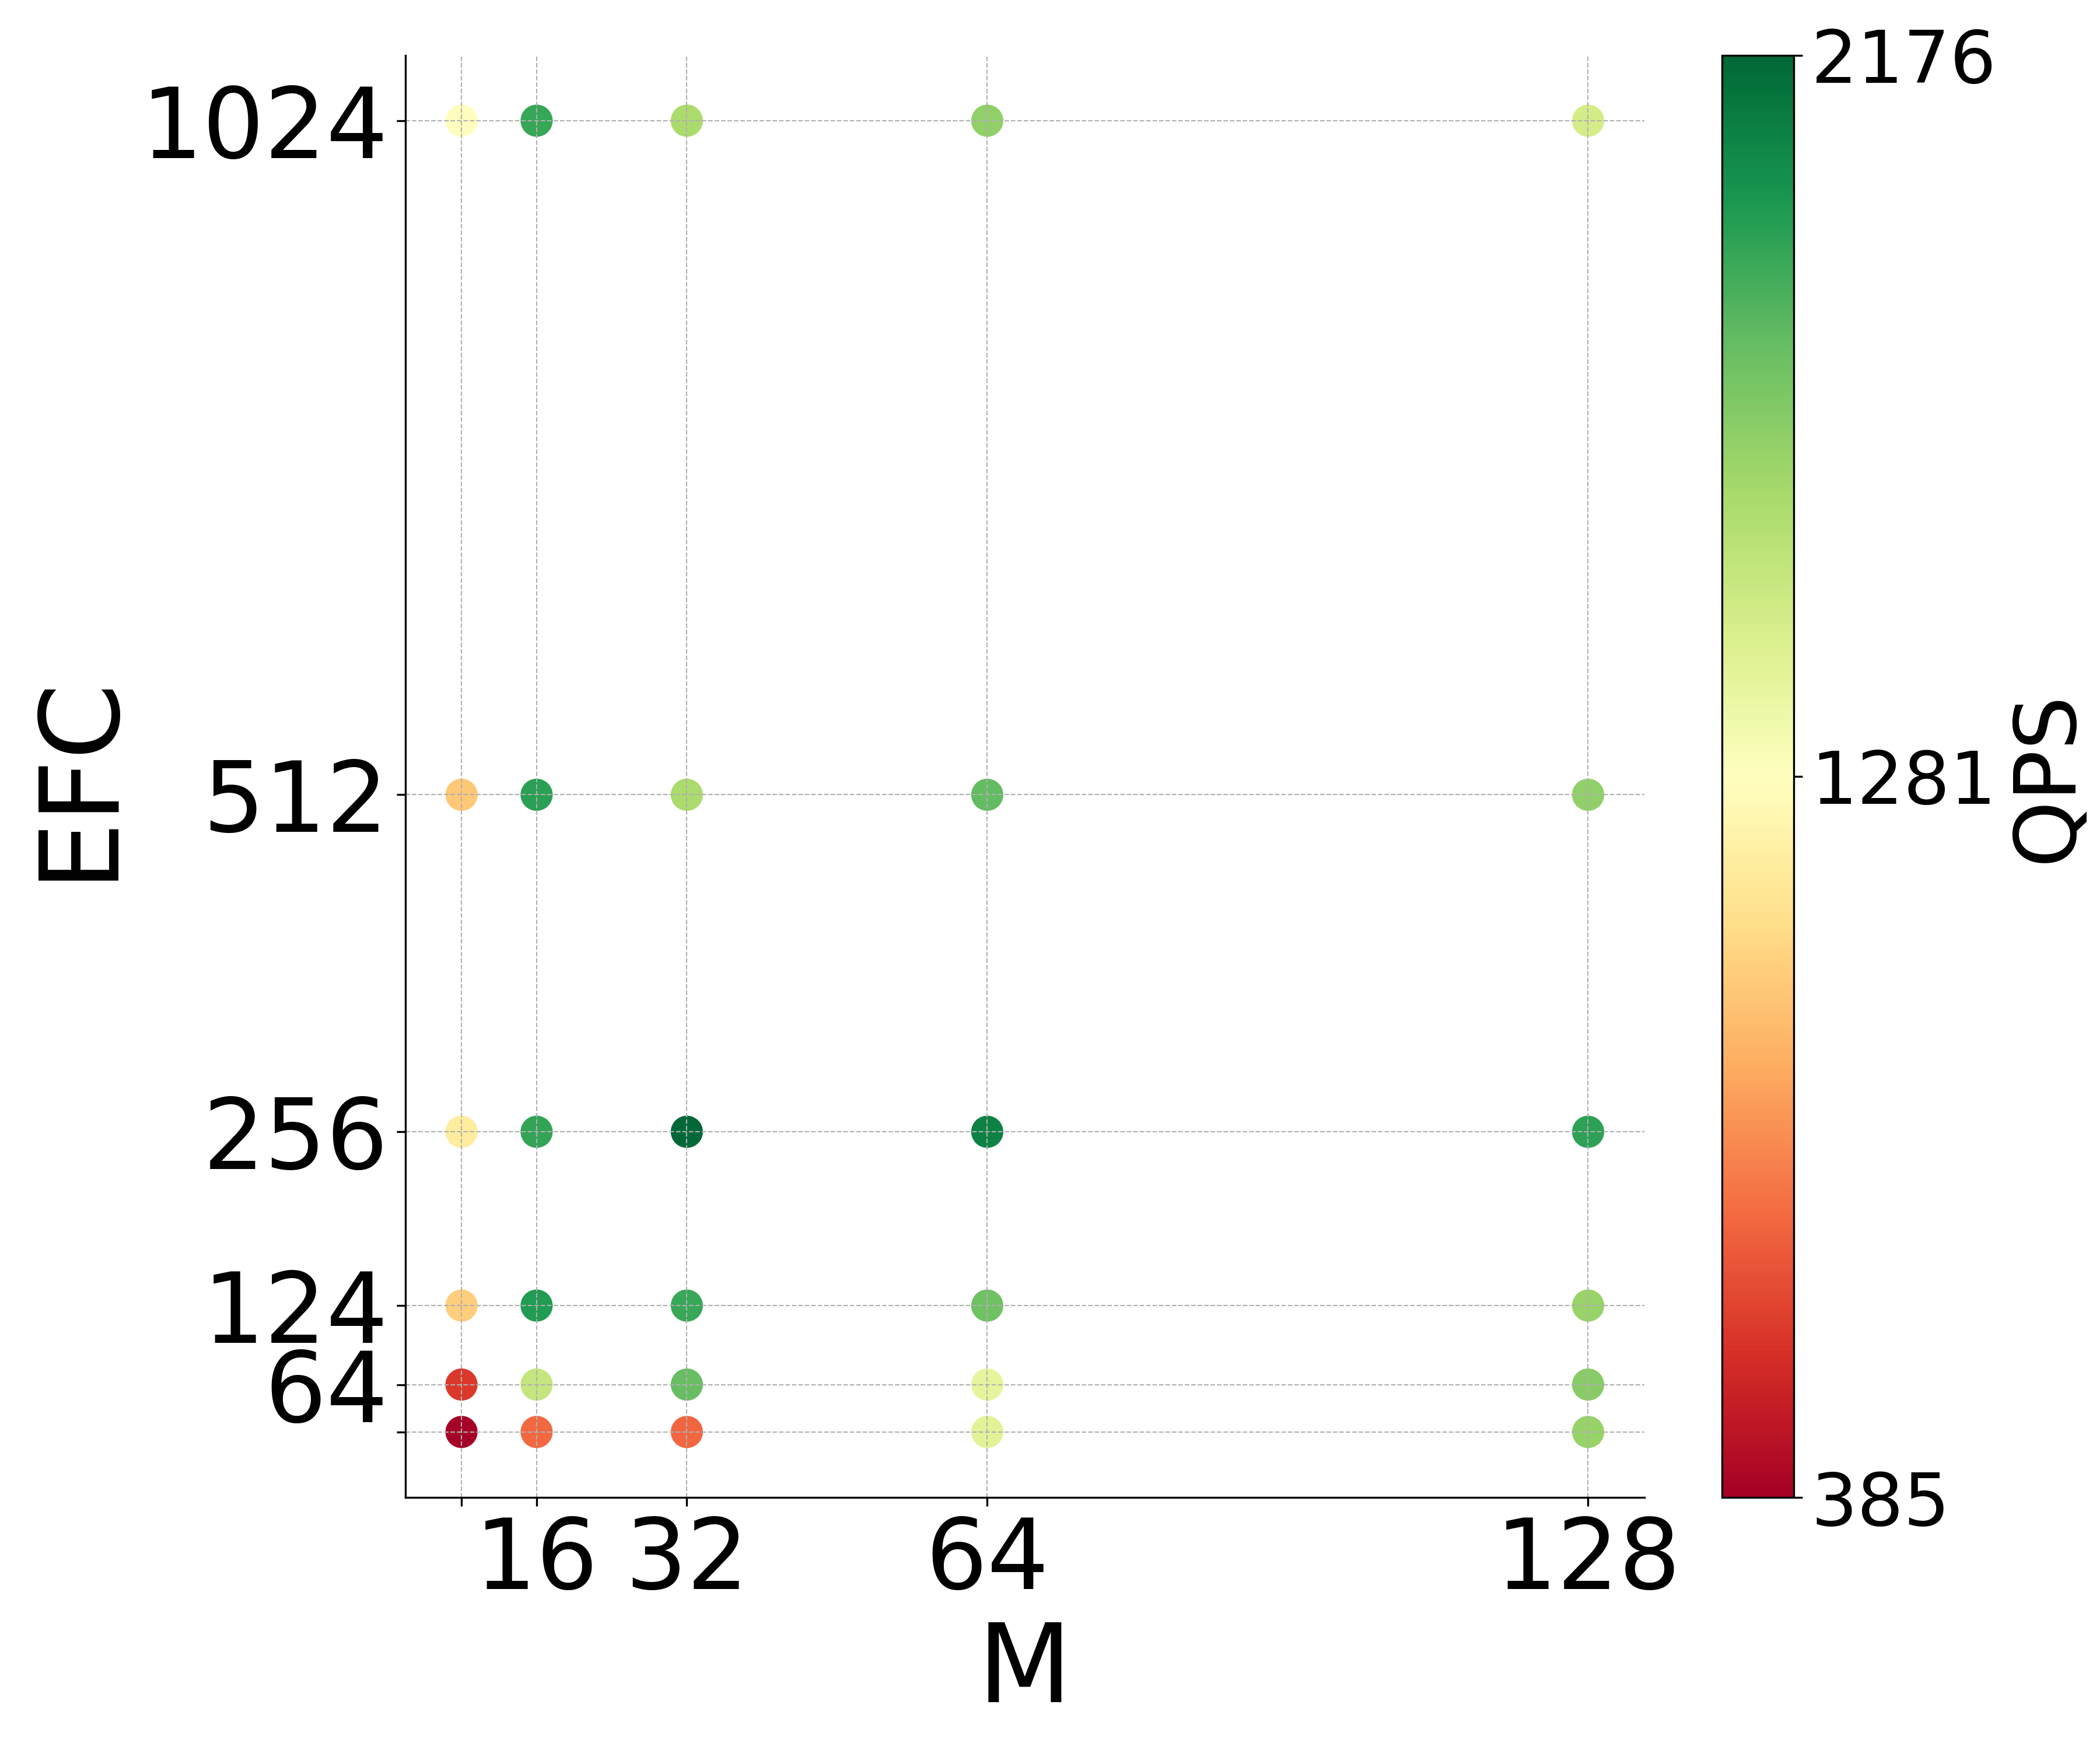
\includegraphics[width=0.7\linewidth]{img/Experiments/search/parametershnsw.png}
    \caption{Indexing Parameters Impact on Search Efficiency at 0.99 recall}
    \label{fig:prmhnsw}
\end{figure}

In Figure ~\ref{fig:prmhnsw} above (where green means best and red means worst), we compare search performance at
0.99 recall for 100 queries on HNSW indices built with different outdegrees (M, ranging from 8 to 128) and beam widths (EFC,
ranging from 32 to 1024). At low M (8), high recall requires a high EFC during search. Increasing EFC during indexing improves the
quality of neighborhood candidates, which is critical for diversification approaches like HNSW, ELPIS, or VAMANA. However,
beyond EFC=128, search efficiency does not improve further, as more neighbors are required per node. Increasing both M and EFC
to their maximums is not advisable, as high outdegree leads to large neighborhood sets, rendering Neighbor Diversification pruning
ineffective. Besides, high values of M or EFC increase indexing time; for instance, M=128 and EFC=1024 is 28x more expensive
than M=8, EFC=32, and 23x more expensive than M=32, EFC=256. Increasing both parameters increases indexing time due to
larger beam widths during insertion and more neighbors to compare during routing. Tuning both parameters can be time-consuming,
especially on large datasets. Therefore, for HNSW and other methods that use a maximum outdegree and beam width as indexing
parameters, we tune the parameters by selecting the best values from a defined range. This range is chosen based on literature and/or from our experiments on previous similar datasets with comparable hardness and/or size.

\section*{Parameters}

We list the parameters for each method in the following tables. For datasets of similar hardness, we find that similar indexing parameters work in both cases. We made changes to the indexing parameters usually due to hardness changes and the size of the dataset.

Our choice of parameters is made based on the performance at high recall (0.99). For the influence of the parameters on graph search.


\begin{table}[h!]
\centering
\caption{Parameters for Deep Dataset}
\scriptsize % Reduce font size further
\begin{tabularx}{\textwidth}{lCCCCC}
\toprule
\textbf{Method} & \textbf{Parameters} & \textbf{1M} & \textbf{25GB} & \textbf{100GB} & \textbf{1B} \\
\midrule
\textbf{HNSW} & M, EFC & 30, 400 & 30, 600 & 50, 800 & 40, 1000 \\
\textbf{VAMANA} & R, L, C, $\alpha$ & 60, 128, 400, 1.2 & 60, 128, 600, 1.2 & 60, 128, 800, 1.2 & 60, 128, 800, 1.2 \\
\textbf{ELPIS} & M, EFC, LS & 20, 300, 0.06 & 24, 300, 0.06 & 30, 400, 0.06 & 40, 600, 0.06 \\
\textbf{NSG} & R, L, C & 60, 128, 400 & 60, 128, 600 & & \\
\textbf{SSG} & R, L, A & 60, 400, 60 & 60, 600, 60 & & \\
\textbf{HCNNG} & R, NC, SC & 3, 30, 500 & 3, 30, 800 & & \\
\textbf{NGT} & e, Loutdeg, S, Moutdeg & 0.1, 10, 20, 40 & 0.1, 10, 30, 60 & & \\
\textbf{SPTAG} & NTree, indeg, TPTnum, TPTLS, ref & 6, 64, 50, 2K, 6 & 6, 64, 50, 3K, 6 & & \\
\textbf{LSHAPG} & M, EFC, NH, LD & 30, 400, 2, 16 & 30, 600, 2, 16 & & \\
\textbf{EFANNA/KGRAPH} & K, mlevel, Ntrees, L, R, S & 64, 6, 6, 256, 256, 8 & 80, 8, 8, 256, 256, 10 & & \\
\textbf{DPG} & K, L, Iter, R, S & 40, 80, 12, 60, 20 & 60, 100, 12, 60, 20 & & \\
\bottomrule
\end{tabularx}
\end{table}


\begin{table}[h!]
\centering
\caption{Parameters for Sift Dataset}
\scriptsize
\begin{tabularx}{\textwidth}{lCCCCC}
\toprule
\textbf{Method} & \textbf{Parameters} & \textbf{1M} & \textbf{25GB} & \textbf{100GB} & \textbf{1B} \\
\midrule
\textbf{HNSW} & M, EFC & 30, 400 & 30, 600 & 50, 800 & 40, 1000 \\
\textbf{VAMANA} & R, L, C, $\alpha$ & 60, 128, 400, 1.2 & 60, 128, 600, 1.2 & 60, 128, 800, 1.2 & 60, 128, 800, 1.2 \\
\textbf{ELPIS} & M, EFC, LS & 20, 300, 0.06 & 24, 300, 0.06 & 30, 400, 0.06 & 40, 600, 0.06 \\
\textbf{NSG} & R, L, C & 60, 128, 400 & 60, 128, 600 & & \\
\textbf{SSG} & R, L, A & 60, 400, 60 & 60, 600, 60 & & \\
\textbf{HCNNG} & R, NC, SC & 3, 30, 500 & 3, 30, 800 & & \\
\textbf{NGT} & e, Loutdeg, S, Moutdeg & 0.1, 10, 20, 40 & 0.1, 10, 30, 60 & & \\
\textbf{SPTAG} & NTree, indeg, TPTnum, TPTLS, ref & 6, 64, 50, 2K, 6 & 6, 64, 50, 3K, 6 & & \\
\textbf{LSHAPG} & M, EFC, NH, LD & 30, 400, 2, 16 & 30, 600, 2, 16 & & \\
\textbf{EFANNA/KGRAPH} & K, mlevel, Ntrees, L, R, S & 64, 6, 6, 256, 256, 8 & 80, 8, 8, 256, 256, 10 & & \\
\textbf{DPG} & K, L, Iter, R, S & 40, 80, 12, 60, 20 & 60, 100, 12, 60, 20 & & \\
\bottomrule
\end{tabularx}
\end{table}


\begin{table}[h!]
\centering
\caption{Parameters for SALD Dataset}
\scriptsize
\begin{tabularx}{\textwidth}{lCCCC}
\toprule
\textbf{Method} & \textbf{Parameters} & \textbf{1M} & \textbf{25GB} & \textbf{100GB} \\
\midrule
\textbf{HNSW} & M, EFC & 36, 480 & 36, 720 & 60, 960 \\
\textbf{VAMANA} & R, L, C, $\alpha$ & 72, 154, 480, 1.2 & 72, 154, 720, 1.2 & 72, 154, 960, 1.2 \\
\textbf{ELPIS} & M, EFC, LS & 24, 360, 0.06 & 29, 360, 0.06 & 36, 480, 0.06 \\
\textbf{NSG} & R, L, C & 72, 154, 480 & 72, 154, 720 & \\
\textbf{SSG} & R, L, A & 72, 480, 72 & 72, 720, 72 & \\
\textbf{HCNNG} & R, NC, SC & 4, 36, 600 & 4, 36, 960 & \\
\textbf{NGT} & e, Loutdeg, S, Moutdeg & 0.1, 12, 24, 48 & 0.1, 12, 36, 72 & \\
\textbf{SPTAG} & NTree, indeg, TPTnum, TPTLS, ref & 7, 77, 60, 2K, 7 & 7, 77, 60, 3K, 7 & \\
\textbf{LSHAPG} & M, EFC, NH, LD & 36, 480, 2, 19 & 36, 720, 2, 19 & \\
\textbf{EFANNA/KGRAPH} & K, mlevel, Ntrees, L, R, S & 77, 7, 7, 308, 308, 9 & 96, 10, 10, 308, 308, 12 & \\
\textbf{DPG} & K, L, Iter, R, S & 48, 96, 14, 72, 24 & 72, 120, 14, 72, 24 & \\
\bottomrule
\end{tabularx}
\end{table}

\begin{table}[h!]
\centering
\caption{Parameters for SEISMIC Dataset}
\scriptsize
\begin{tabularx}{\textwidth}{lCCCC}
\toprule
\textbf{Method} & \textbf{Parameters} & \textbf{1M} & \textbf{25GB} & \textbf{100GB} \\
\midrule
\textbf{HNSW} & M, EFC & 60, 800 & 60, 1200 & 100, 1600 \\
\textbf{VAMANA} & R, L, C, $\alpha$ & 120, 256, 800, 1.2 & 120, 256, 1200, 1.2 & 120, 256, 1600, 1.2 \\
\textbf{ELPIS} & M, EFC, LS & 40, 600, 0.06 & 48, 600, 0.06 & 60, 800, 0.06 \\
\textbf{NSG} & R, L, C & 120, 256, 800 & 120, 256, 1200 & \\
\textbf{SSG} & R, L, A & 120, 800, 120 & 120, 1200, 120 & \\
\textbf{HCNNG} & R, NC, SC & 6, 60, 1000 & 6, 60, 1600 & \\
\textbf{NGT} & e, Loutdeg, S, Moutdeg & 0.1, 20, 40, 80 & 0.1, 20, 60, 120 & \\
\textbf{SPTAG} & NTree, indeg, TPTnum, TPTLS, ref & 12, 128, 100, 4K, 12 & 12, 128, 100, 6K, 12 & \\
\textbf{LSHAPG} & M, EFC, NH, LD & 60, 800, 2, 32 & 60, 1200, 2, 32 & \\
\textbf{EFANNA/KGRAPH} & K, mlevel, Ntrees, L, R, S & 128, 12, 12, 512, 512, 16 & 160, 16, 16, 512, 512, 20 & \\
\textbf{DPG} & K, L, Iter, R, S & 80, 160, 24, 120, 40 & 120, 200, 24, 120, 40 & \\
\bottomrule
\end{tabularx}
\end{table}


\chapter{Empirical Analysis of the Theoretical Complexity of Beam search}
\label{appendix:beamsearch}
Beam search, introduced by Raj Reddy in 1977, is a core algorithm widely used across various fields, including speech recognition, machine translation, and natural language processing. It operates by exploring a restricted number of hypotheses, referred to as the "beam," improving efficiency compared to exhaustive search approaches. However, beam search trades off completeness and optimality for speed, as it may prune potential goal states, and thus does not always guarantee finding the best solution. The time complexity of beam search is determined by factors such as the beam width and the maximum allowable path length in the graph. When applied to proximity graphs, as used in spatial data analysis, beam search efficiently explores nearby nodes or edges, making it highly versatile across different domains.

The time complexity of beam search is described by the following formula:

\[
\text{Time Complexity} = O(B \times m \times T) \quad (\text{Eq. 4})
\]

Where \( B \) denotes the beam width, \( m \) represents the average branching factor (or average out-degree in graph search), and \( T \) indicates the maximum path length allowed within the graph. In the worst case, \( T \) is equivalent to the graph's diameter, representing the longest possible path. This formula captures the computational cost of beam search, factoring in the beam width, average out-degree, and graph diameter. However, because the search accuracy for a given beam width is not guaranteed, the exact time complexity can only be approximated by running a search on a query set to determine the necessary beam width for a target accuracy. Sometimes, the differences in beam widths between methods may have a greater impact on time complexity than variations in out-degree or diameter. It is also worth noting that different seed selection strategies can affect time complexity, especially when the number of nearest neighbors required is small.

Below, we provide an analysis of the theoretical time complexity and its alignment with the empirical performance of four state-of-the-art graph-based algorithms. For each method, the graph is built with maximum out-degrees of 40, 40, 50, and 60 for the datasets Deep1M, Deep2M, Deep4M, and Deep8M, respectively. The purpose is to examine how the theoretical time complexity corresponds to the empirical performance of the methods, both in terms of time and the number of distance calculations. All measurements are taken for a target accuracy of 0.99.

\begin{figure}
\centering
\begin{subfigure}{0.45\textwidth}
  \centering
  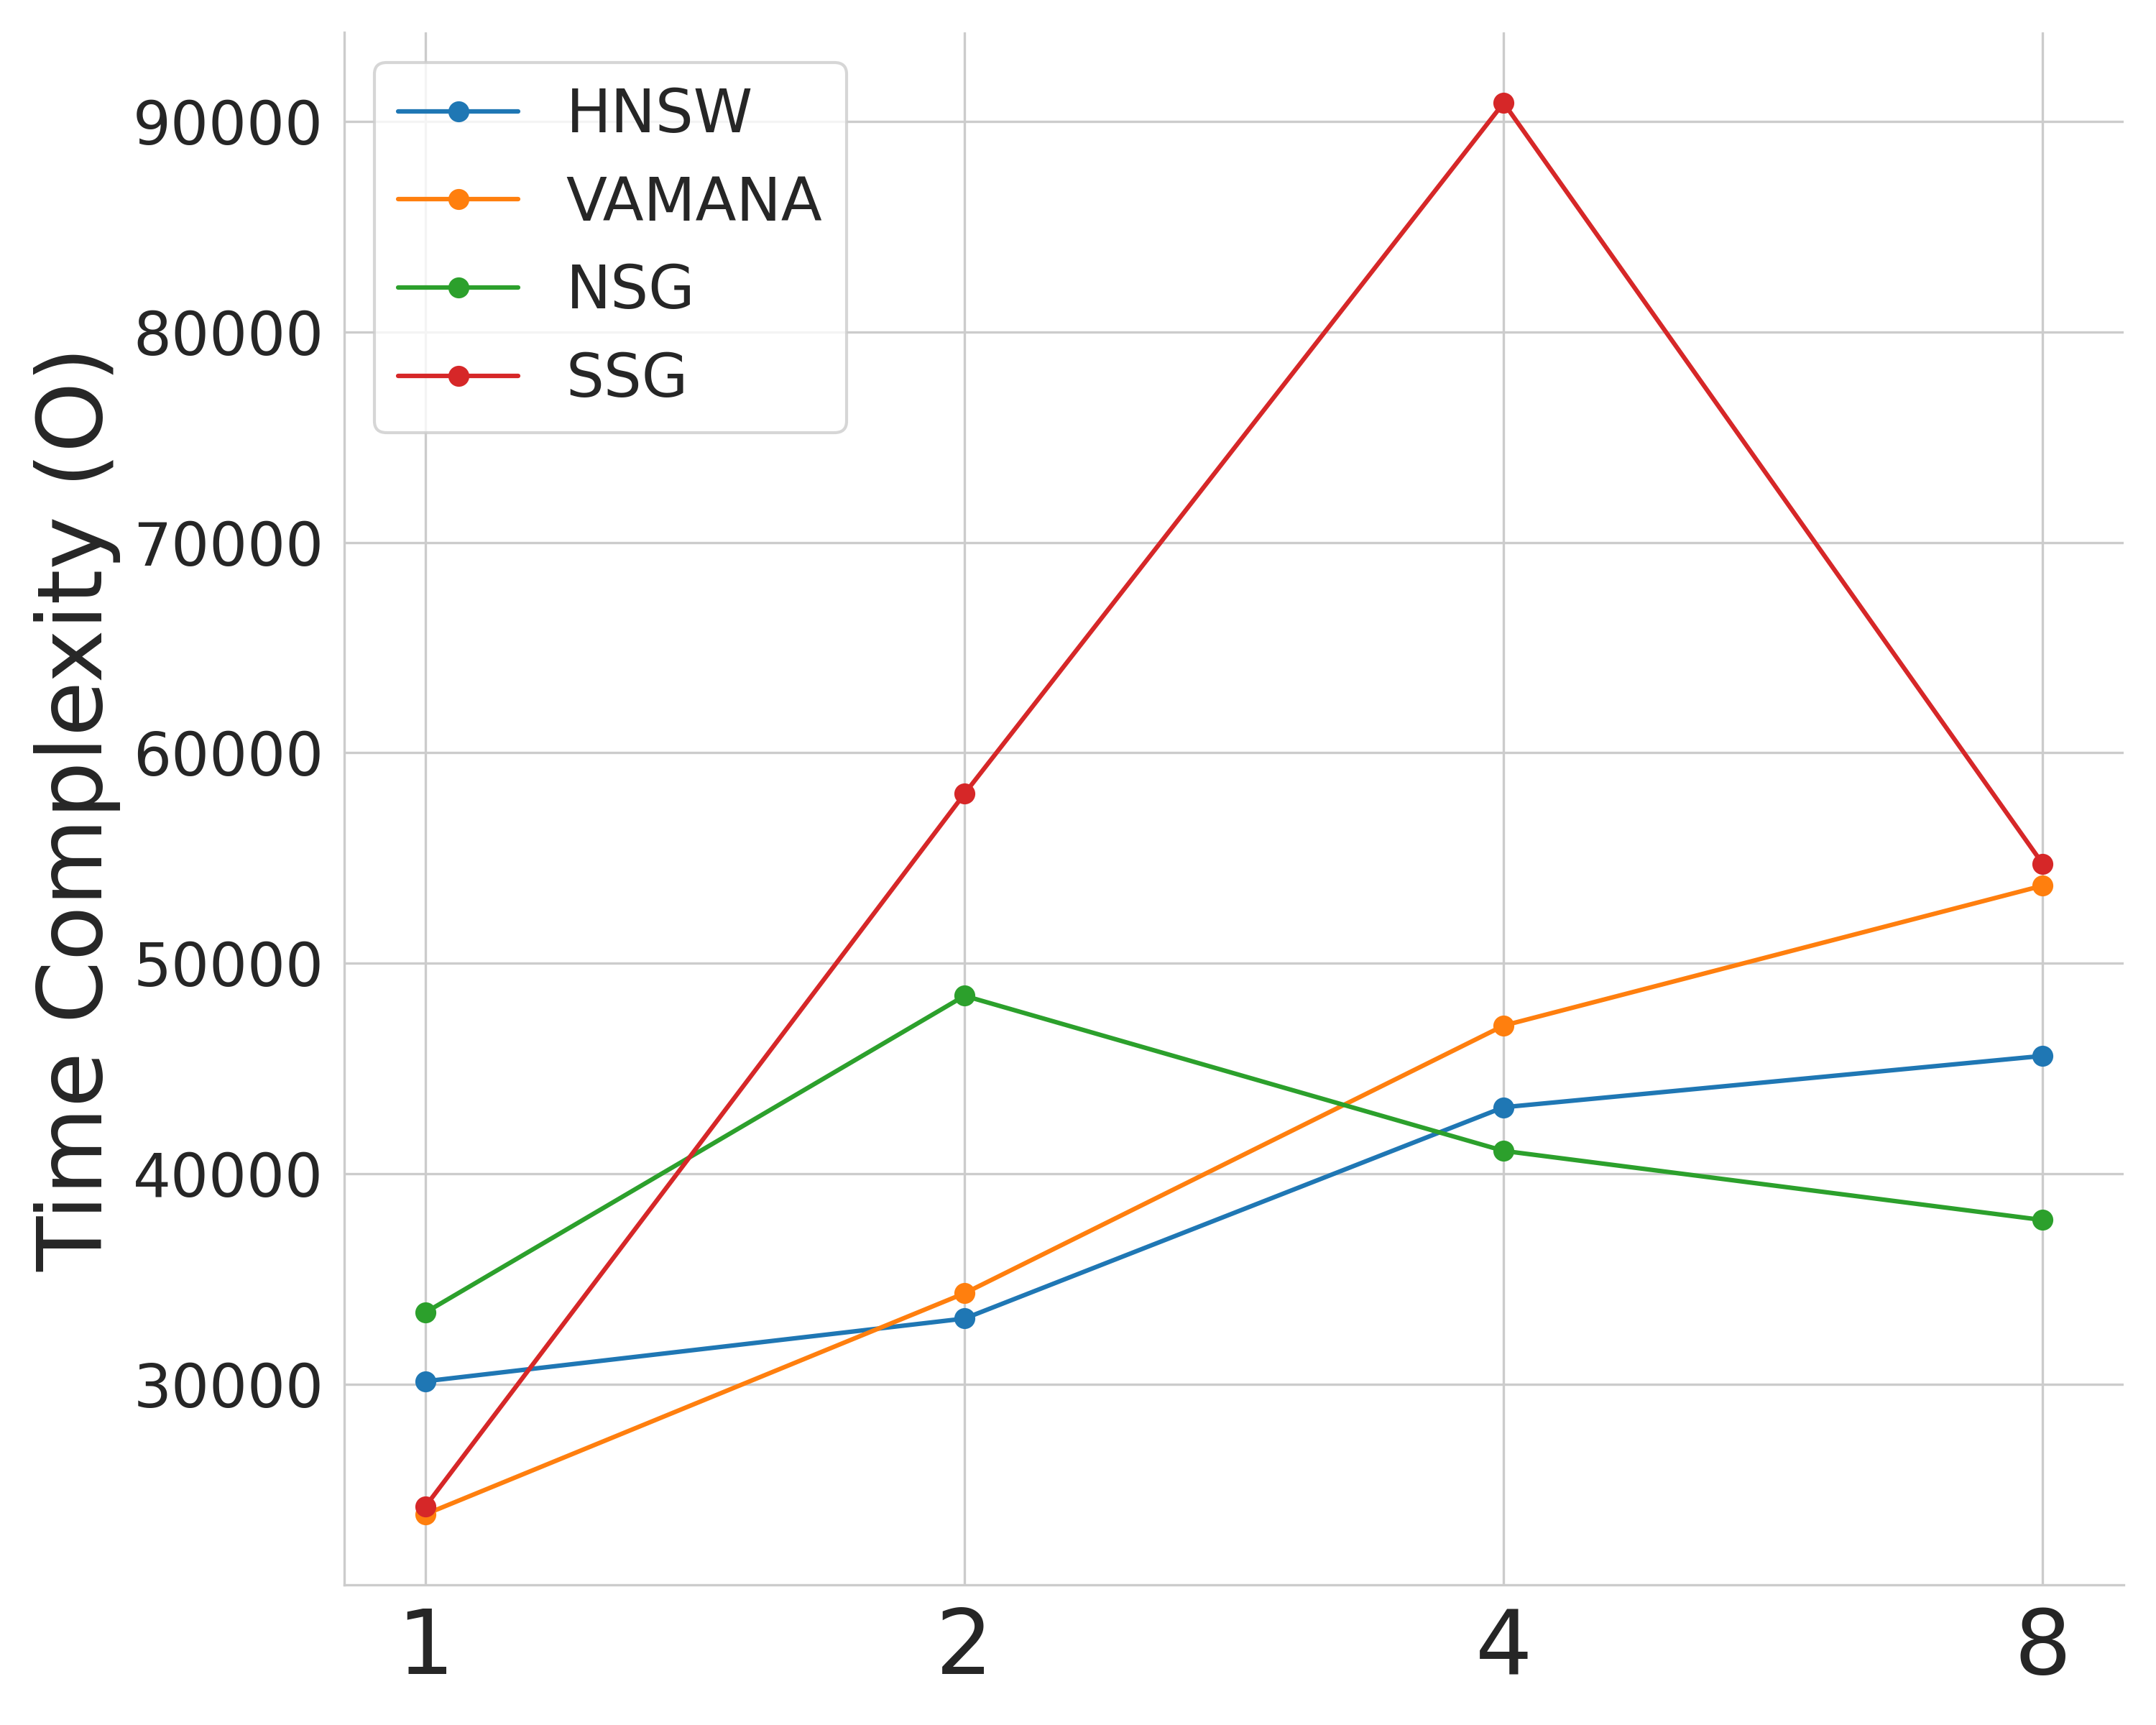
\includegraphics[width=\linewidth]{../img/Experiments/BSC/complexity_size.png}
  \caption{Theoretical Time Complexity}
  \label{fig:cno}
\end{subfigure}
\hfill
\begin{subfigure}{0.45\textwidth}
  \centering
  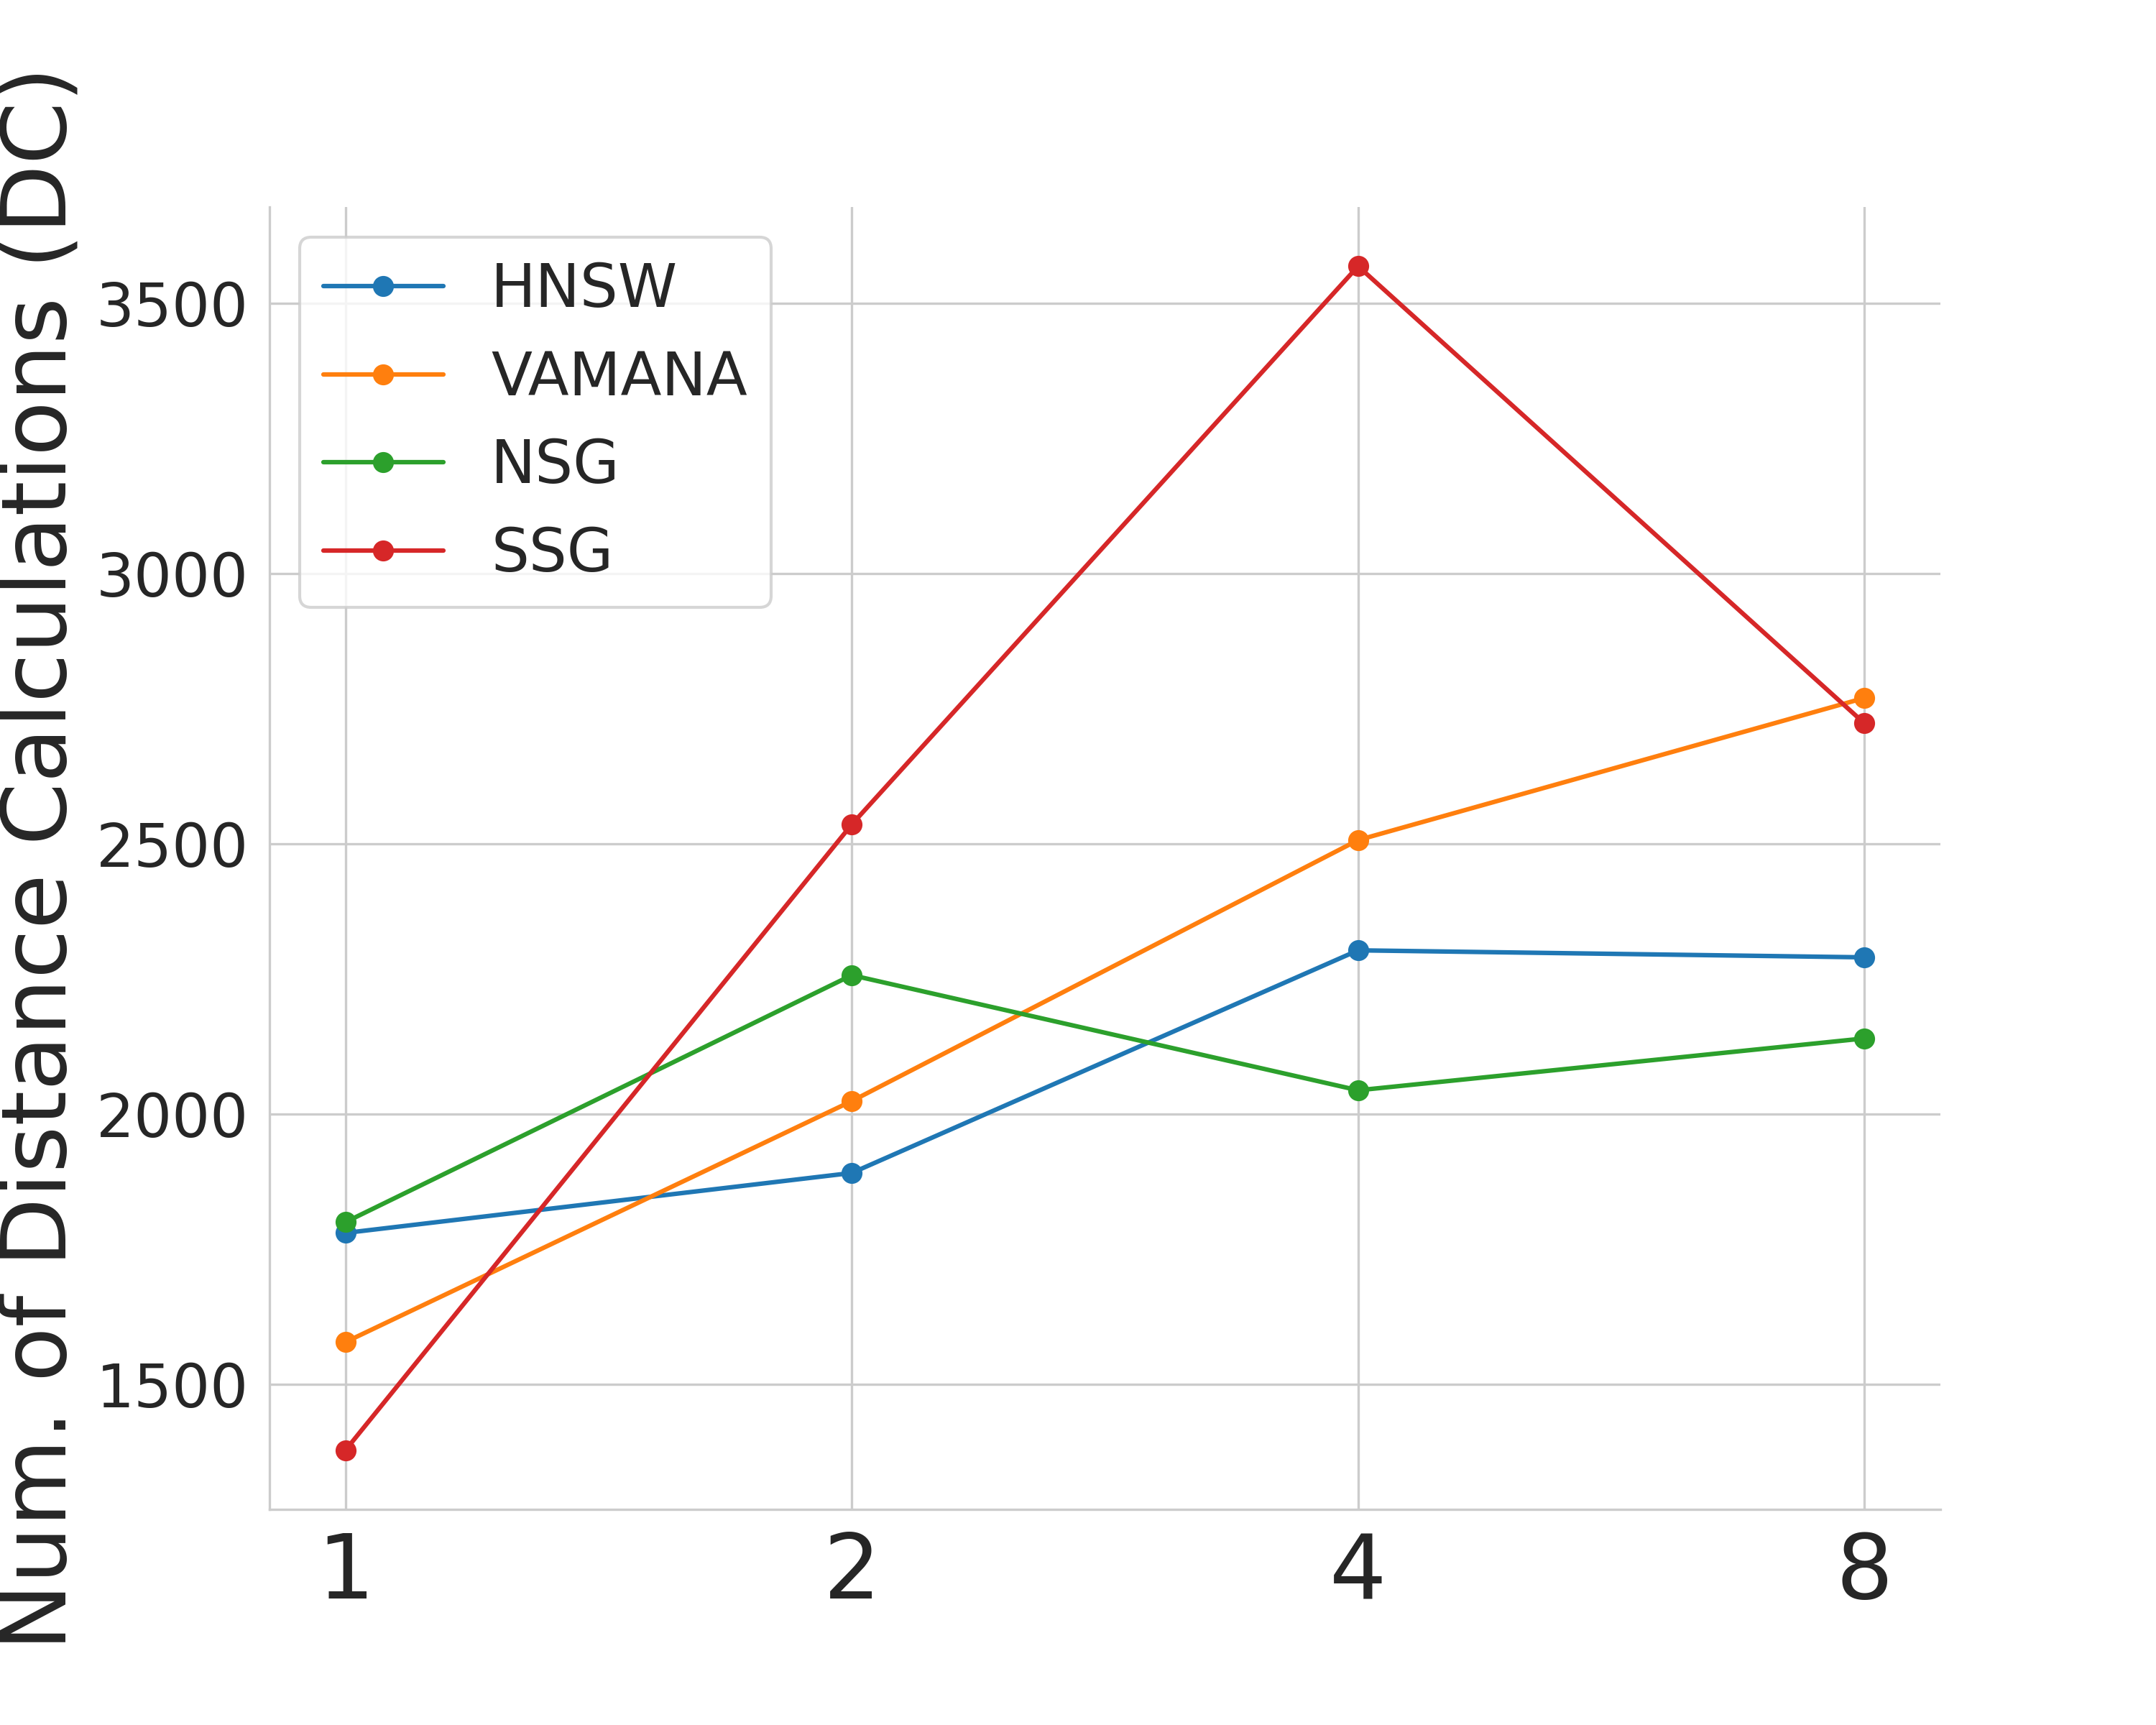
\includegraphics[width=\linewidth]{../img/Experiments/BSC/dc_size.png}
  \caption{Empirical efficiency}
  \label{fig:dc}
\end{subfigure}
\caption{Theoretical and empirical beams search efficiency across different deep1b dataset sizes}
\label{fig:ndc_no_size_plots}
\end{figure}

In Figure ~\ref{fig:ndc_no_size_plots}, we illustrate how the theoretical time complexity of the beam search aligns with the algorithm efficiency, specifically the number of distance calculations across different dataset sizes. As the dataset size increases, we can observe an improvement in the approximation of the empirical complexity (comparing 1M to 2M, 4M, and 8M), as the ranking between methods in terms of beam search efficiency is approximated using the beam search time complexity formula in Eq. 4.
In Figure ~\ref{fig:ndc_no_plots}, we present the comparison between the time complexity and search efficiency of four methods for different deep1b dataset scales.

\begin{figure}[htbp]
\centering
\begin{subfigure}{0.24\textwidth}
  \centering
  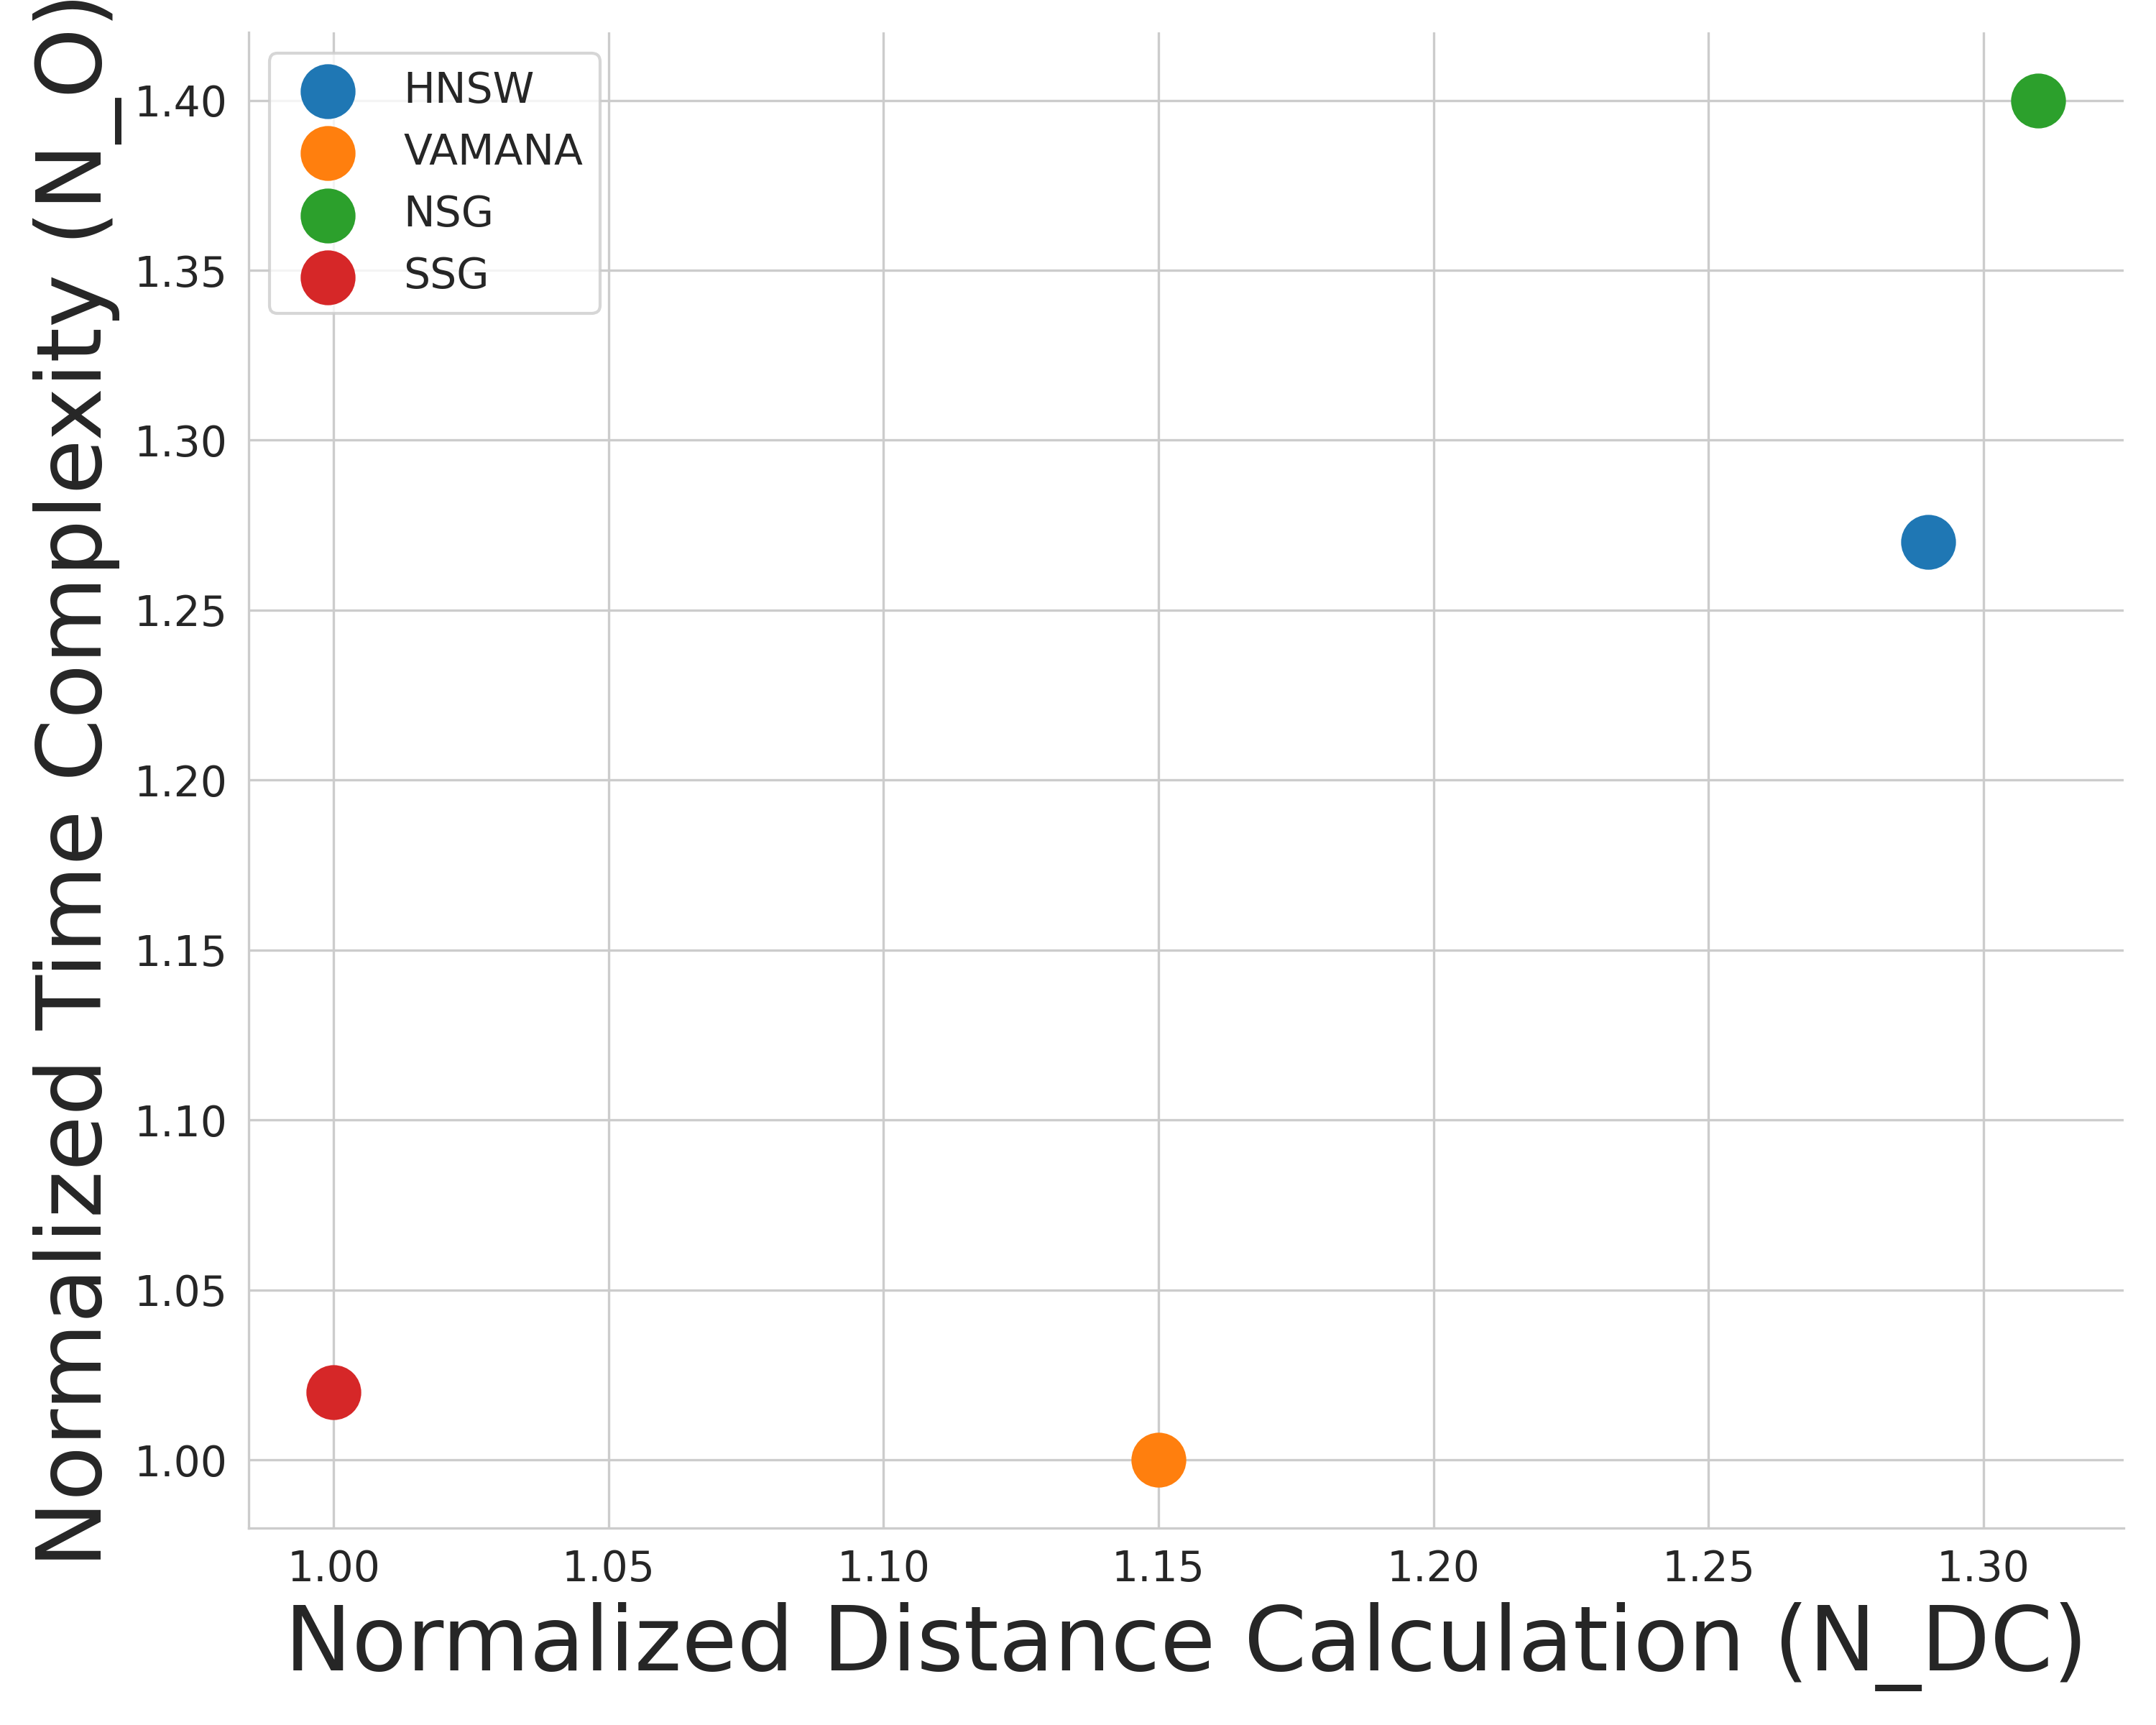
\includegraphics[width=\linewidth]{../img/Experiments/BSC/1_ndc_no.png}
  \caption{Deep1M}
  \label{fig:1_ndc_no}
\end{subfigure}
\hfill
\begin{subfigure}{0.24\textwidth}
  \centering
  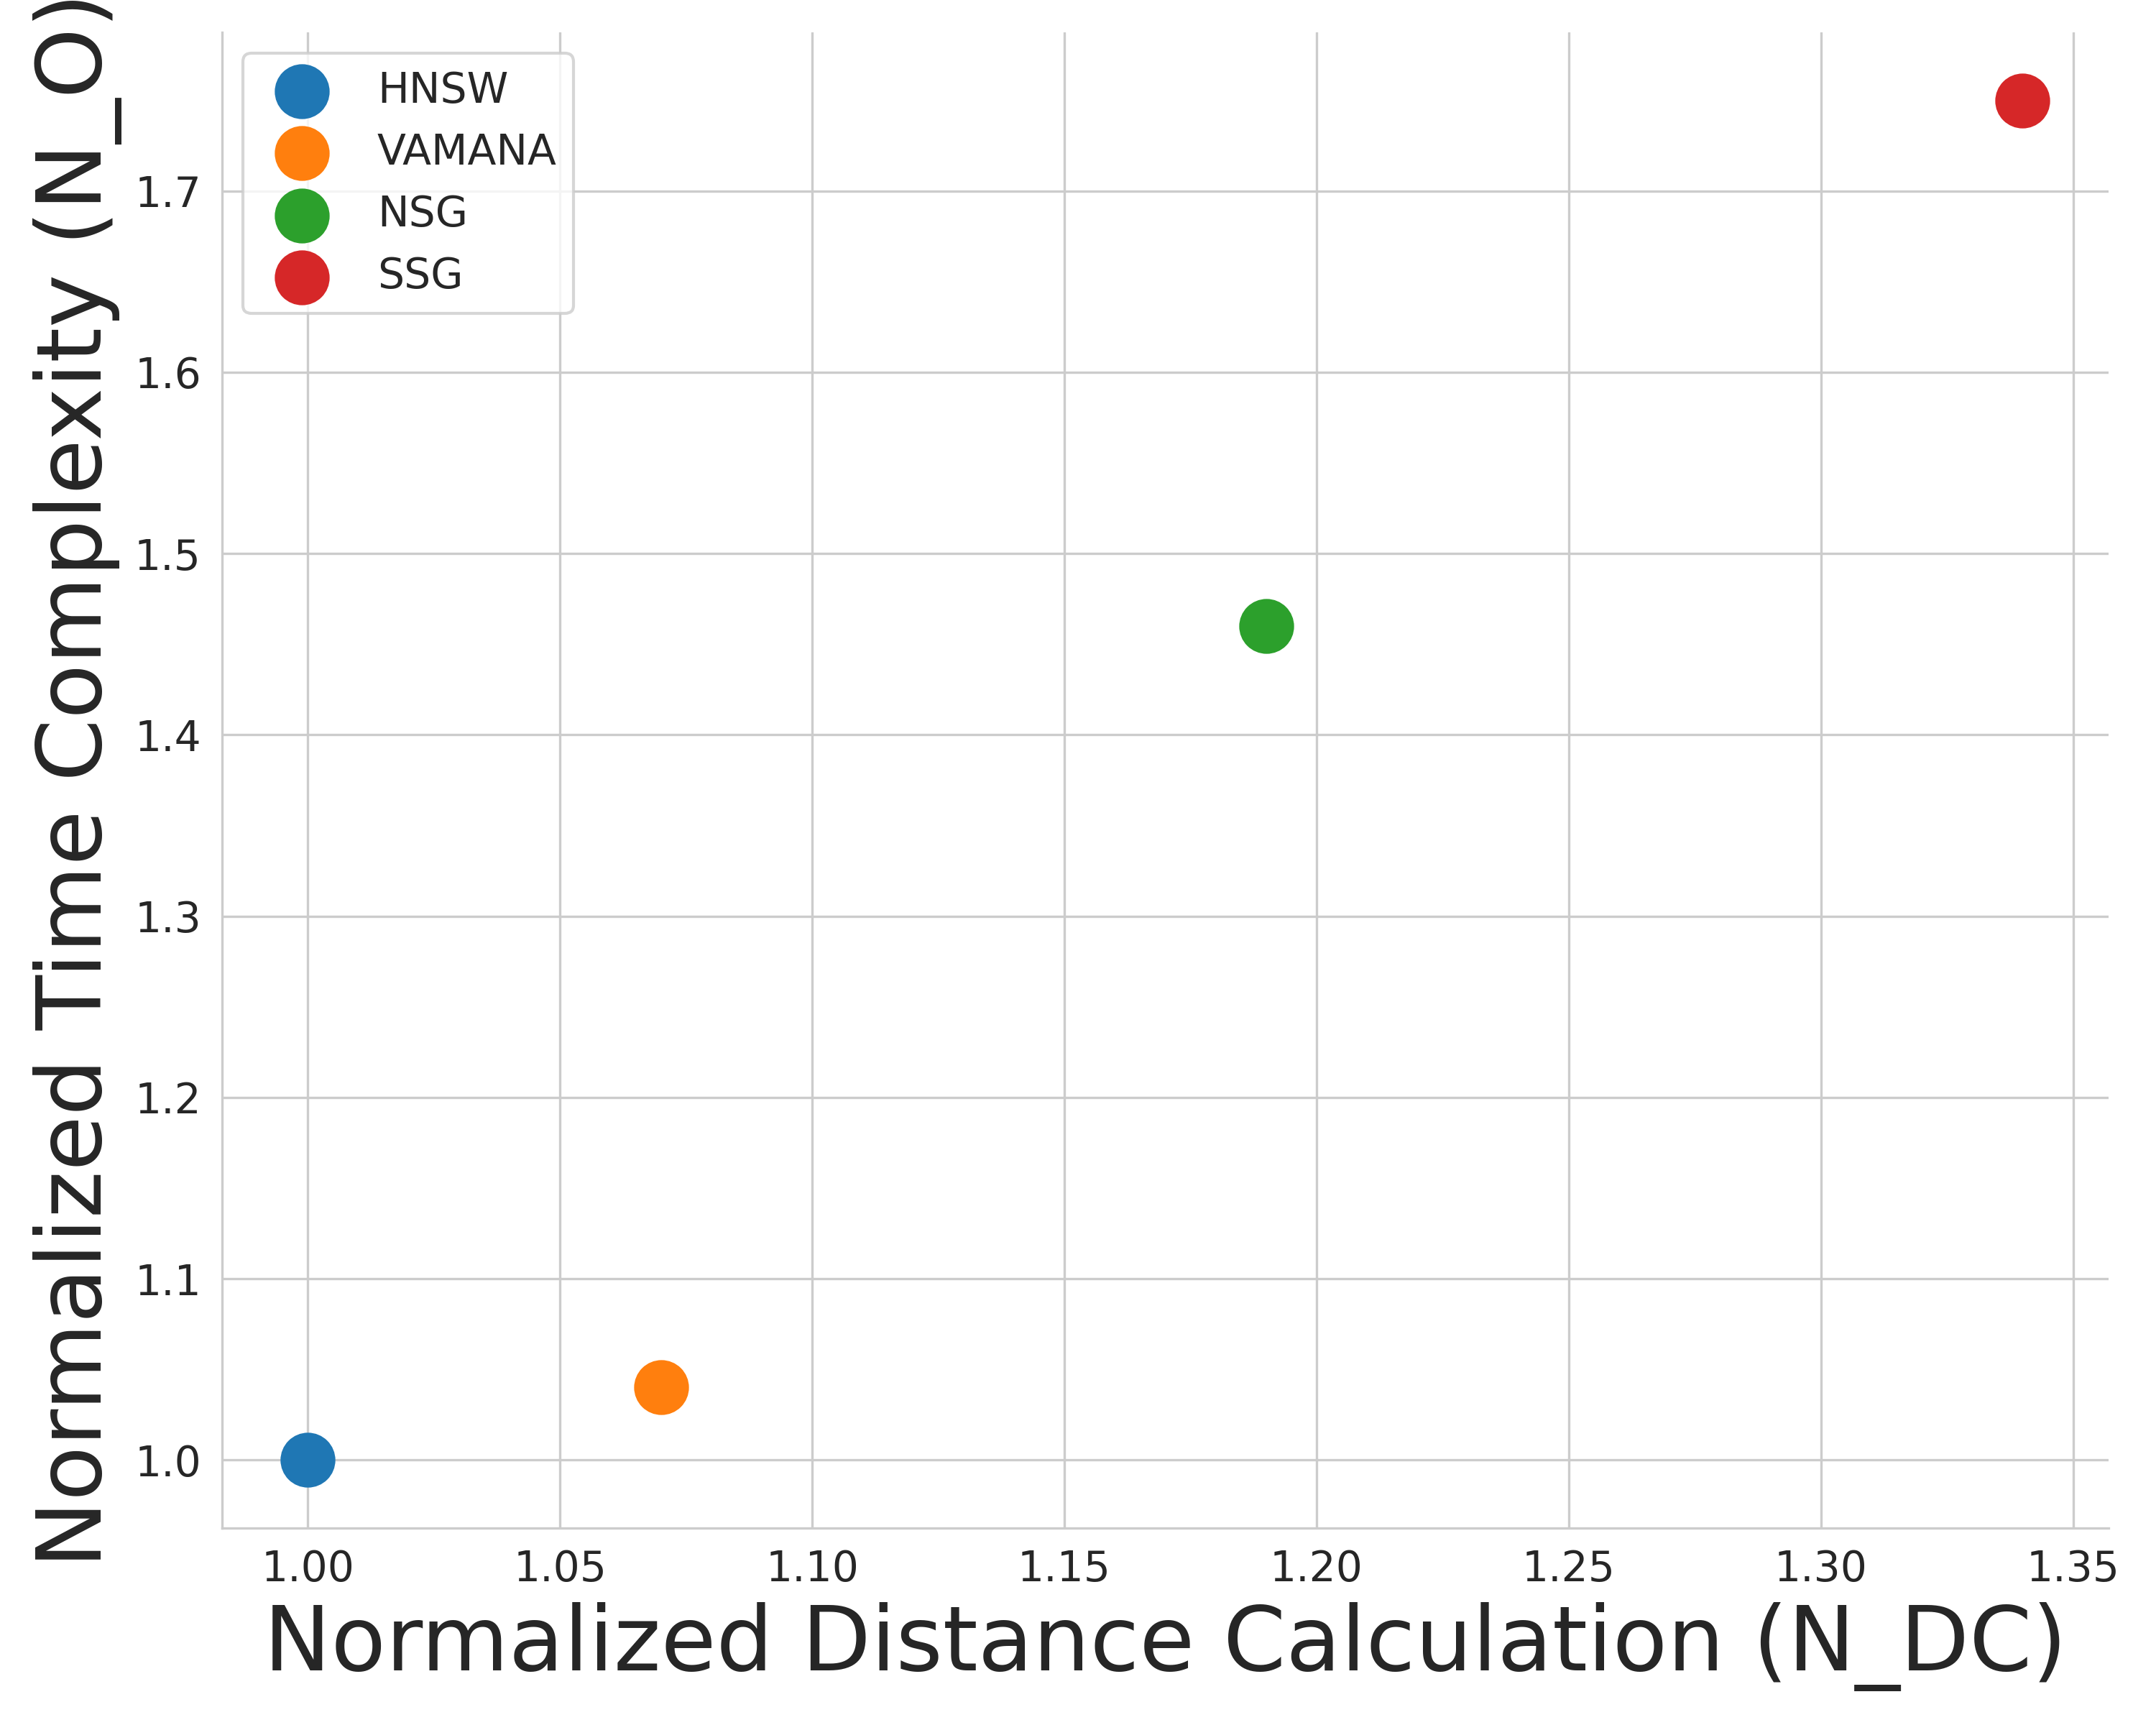
\includegraphics[width=\linewidth]{../img/Experiments/BSC/2_ndc_no.png}
  \caption{Deep2M}
  \label{fig:2_ndc_no}
\end{subfigure}
\begin{subfigure}{0.24\textwidth}
  \centering
  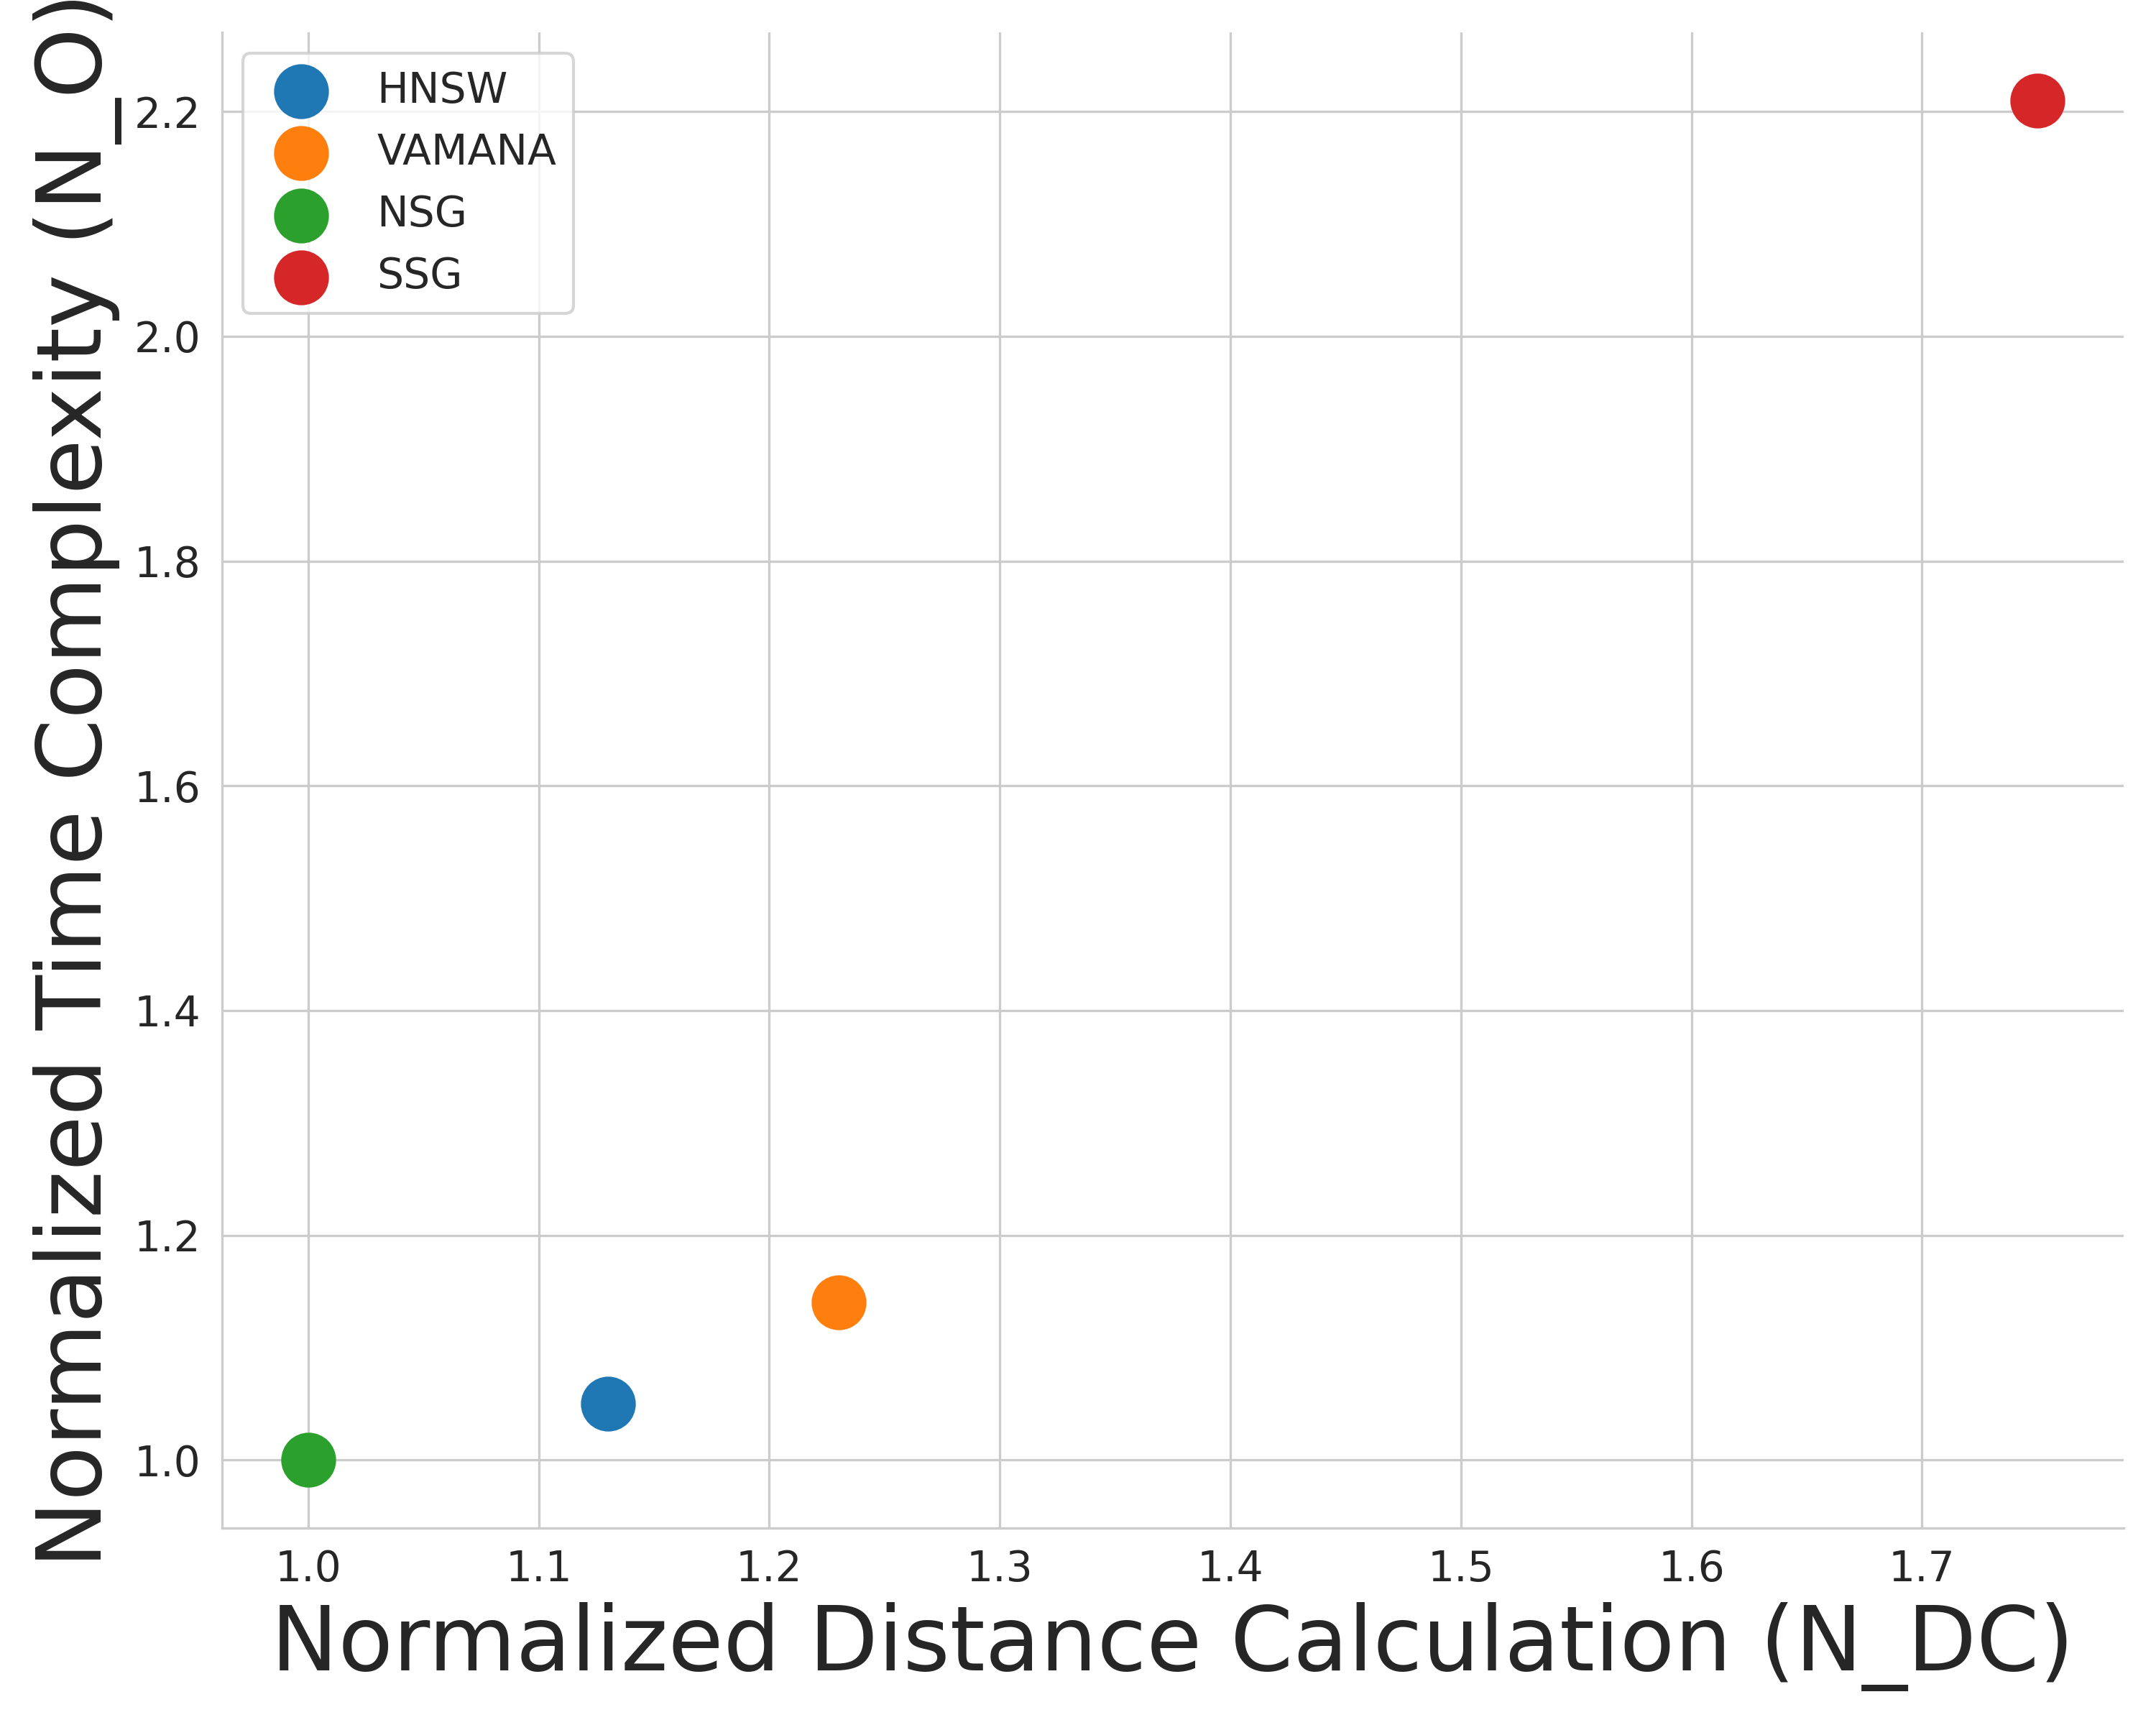
\includegraphics[width=\linewidth]{../img/Experiments/BSC/4_ndc_no.png}
  \caption{Deep4M}
  \label{fig:4_ndc_no}
\end{subfigure}
\hfill
\begin{subfigure}{0.24\textwidth}
  \centering
  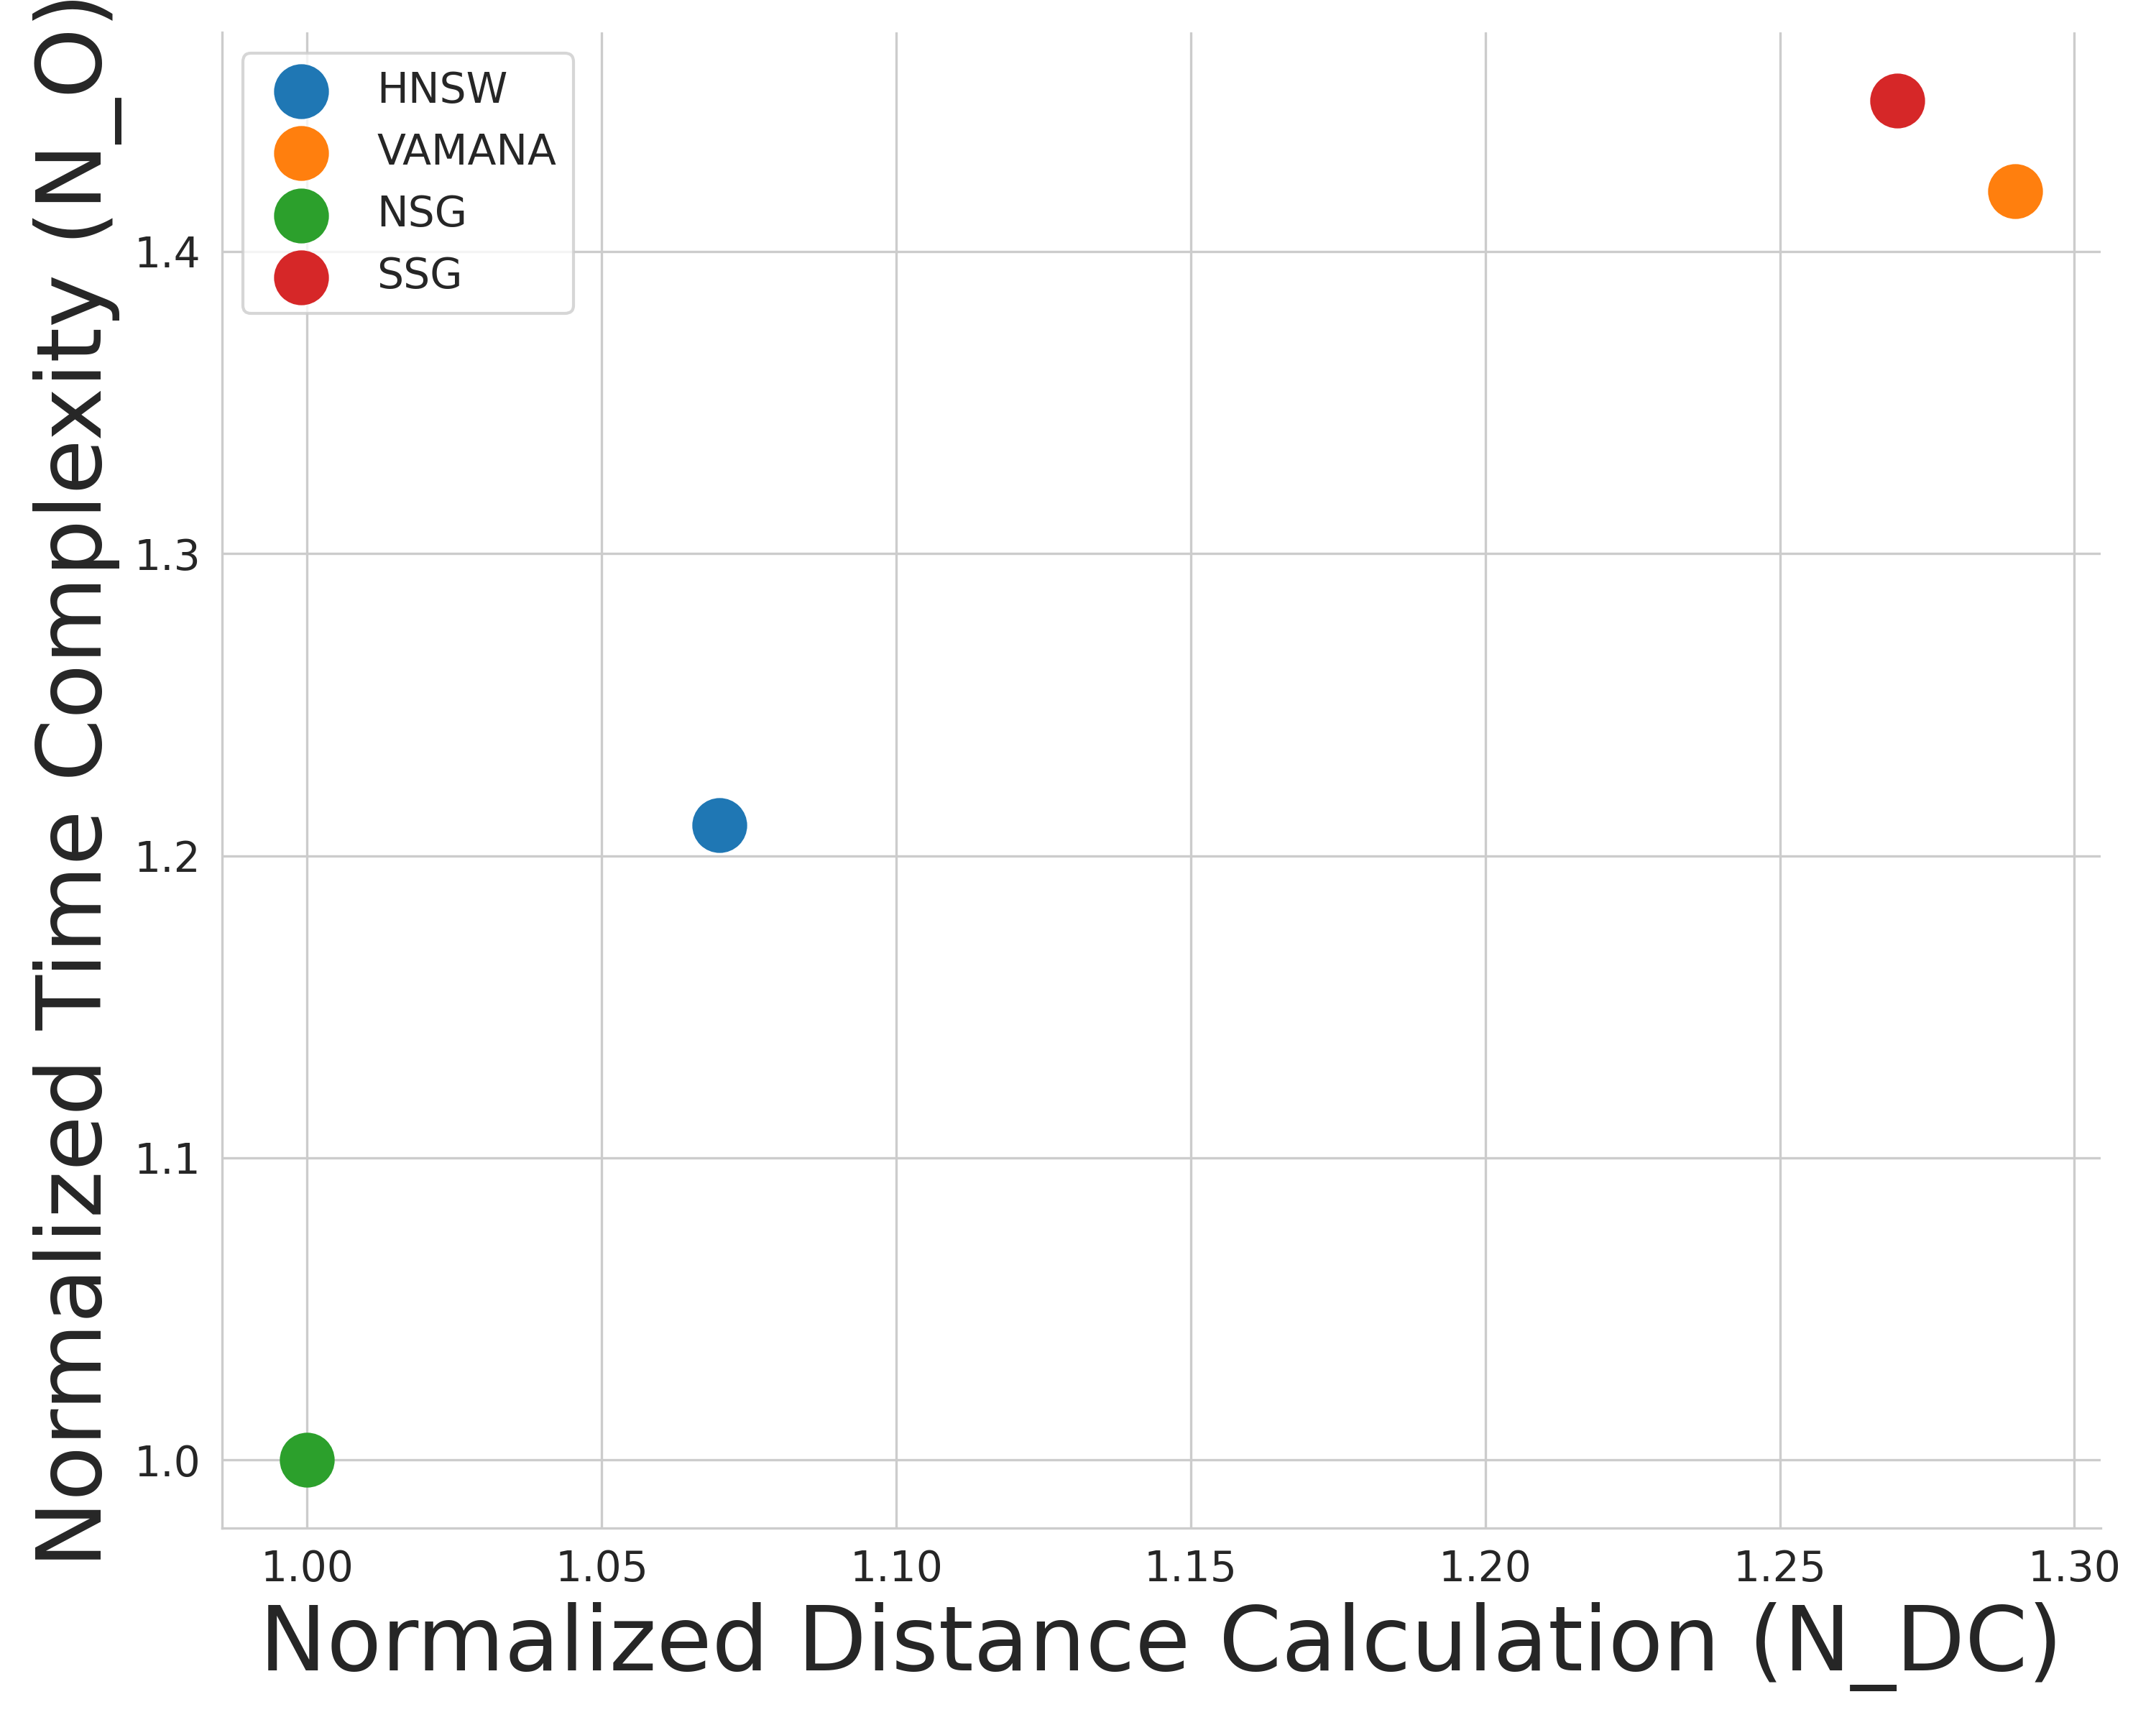
\includegraphics[width=\linewidth]{../img/Experiments/BSC/8_ndc_no.png}
  \caption{Deep8M}
  \label{fig:8_ndc_no}
\end{subfigure}
\caption{Normalized Distance Calculation (N\_DC) vs Normalized Time Complexity (N\_O) across different Deep1B dataset sizes}
\label{fig:ndc_no_plots}
\end{figure}


